در این پوشه به تمام مسیر‌های نرم‌افزار پرداخته شده است.

\begin{figure}[H]
	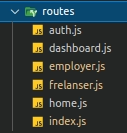
\includegraphics[width=.3\textwidth]{Folders-Files/routes.png}
	\centering
	\caption{ساختار پوشه مسیر}
	\label{fig:folder-routes}
\end{figure}

\subsection{فایل index}
در این فایل تمام آدرس‌های پوشه‌های مسیر برنامه قرار دارد.

\subsection{فایل home}
در این فایل به مسیر صفحه اصلی/اول/خانه پرداخته شده است.

\subsection{فایل auth}
در این فایل به مسیر ورود، ثبت‌نام و خروج پرداخته شده است.

\subsection{فایل dashboard}
در این فایل به مسیر داشبورد کاربر پرداخته شده است.

\subsection{فایل employer}
در این فایل به مسیر داشبورد کارفرما پرداخته شده است.

\subsection{فایل frelanser}
در این فایل به مسیر داشبورد فریلنسر پرداخته شده است.



checkdate
\\
 اعتبارسنجی تاریخ هجری شمسی
\\
توضیحات
\\
bool shcheckdate ( int \$year , int \$month , int \$day );

\begin{minted}{python}
	import numpy as np
	
	def incmatrix(genl1,genl2):
	m = len(genl1)
	n = len(genl2)
	M = None #to become the incidence matrix
	VT = np.zeros((n*m,1), int)  #dummy variable
	
	#compute the bitwise xor matrix
	M1 = bitxormatrix(genl1)
	M2 = np.triu(bitxormatrix(genl2),1) 
	...
\end{minted}

\mint{html}|<h2>Something <b>here</b></h2>|

بررسی اعتبار تاریخی که توسط آرگومان‌های تابع وارد می‌شود.در صورتی که پارامترها به درستی وارد شوند،یک تاریخ معتبر خواهد بود.
\rule{\linewidth}{0.5mm}

پارامترها
\\
\begin{tabular}{|c|c|}
	\hline
	 پارامتر	& توضیحات \\
	\hline
	&  \\
	\hline
	&  \\
	\hline
\end{tabular}

برگردان
\\
در صورتی که تاریخ وارد شده معتبر باشد TRUE در غیر این صورت FALSE خواهد بود.

